%
% ─── CAPITULO 7: VISUALIZACION DE FRACTALES 2D ──────────────────────────────────
%

En el capítulo \ref{chap:visualizacion} introdujimos el uso de WebGL como herramienta de generación de imágenes y estudiamos sus componentes, sin embargo, no olvidemos que nuestro objetivo es la visualización de fractales, donde la característica principal de los mismos es que no se pueden expresar a partir de un conjunto de vértices o líneas, sino que son curvas o superficies totalmente irregulares. Entonces, ¿cómo podemos usar WebGL para graficar imágenes fractales?

A nivel conceptual, una imagen realmente es un conjunto de píxeles con un color asociado. Si identificamos cada píxel con la dupla de números naturales $(x,y)$ formada por el número de fila y de columna que ocupa el píxel, entonces a partir de una función $f$ que a cada pareja le asigne un color, esto es, una terna $(r,g,b)$, podemos obtener una imagen. Fíjese en el ejemplo de la imagen \ref{fig:sintesis-imagenes-f}, donde generamos una imagen de $4\times 2$ píxeles a partir de una función $f$. Si queremos implementar esta síntesis de imágenes mediante una función $f$, podemos programar esta función $f$ y ejecutarla en CPU píxel a píxel de manera secuencial, pero evidentemente sería más rápido y eficiente paralelizar el cálculo de $f$ aprovechando la GPU, de forma que en un mismo instante se pueden estar procesando miles de píxeles en lugar de uno. 

\begin{figure} [ht]
    \centering
    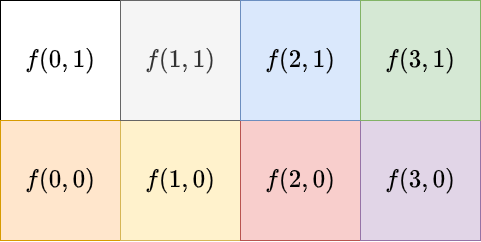
\includegraphics[scale = 0.4]{img/C7/sintesis-imagenes-f.png}
    \caption{Síntesis de una imagen vía una función}
    \label{fig:sintesis-imagenes-f}
\end{figure}


Sin embargo, WebGL está orientado a rasterización, es decir, dadas unas primitivas colorea del color adecuado los píxeles que ocupen estas primitivas, dividiendo las mismas en triángulos. La forma que tenemos por tanto de ejecutar $f$ una vez por cada píxel es rasterizando dos triángulos que ocupen toda la superficie del canvas. Al existir dos primitivas que en conjunto cubren toda la imagen, el fragment shader se ejecutará una vez por cada píxel. Desde el fragment shader podemos acceder a las coordenadas del píxel, y utilizando estas coordenadas y los valores asignados a las variables \verb|varying| y \verb|uniform|, calcular el valor que devuelve la función $f$, asignando así un color a cada píxel, que es precisamente el cometido del fragment shader.

Por tanto, a efectos prácticos, nuestro vertex shader tomará como entrada los vértices $(-1,-1)$, $(1,-1)$, $(1,1)$ y $(-1,1)$ y no aplicará ninguna transformación, pues ya están normalizados en el clip space (teniendo en cuenta que estaríamos visualizando un fragmento del plano $z=0$). Cabe en este momento aclarar que en el ámbito de herramientas de visualización por convenio se suele utilizar la coordenada $Y$ para la altura y la coordenada $Z$ para la profundidad. 

A partir de estos cuatro vértices, en el canvas se visualizarán dos triángulos que completarán la superficie completa del mismo. El vertex shader a partir de ahora será totalmente trivial, pues solo devolverá en la variable \verb|gl_Position| la misma posición que obtiene del buffer de posición.

\begin{lstlisting}
attribute vec2 a_Position;
void main() {
  gl_Position = vec4(a_Position.x, a_Position.y, 0.0, 1.0);
}
\end{lstlisting}

Mientras que, por su parte, el fragment shader podrá acceder a la posición (en coordenadas de dispositivo) del píxel que se está ejecutando mediante la variable \verb|gl_FragCoord| y a partir de estas coordenadas devolver un color en la variable \verb|gl_FragColor|. Es decir, estamos dibujando una escena completa, próximamente un fractal, en dos triángulos. Por ejemplo, las imágenes \ref{fig:julia-intro} y \ref{fig:mandelbrot-intro} son el resultado de esta metodología. 

\begin{comment}

\section{Objetivo}

Procedemos a explicar el objetivo principal de este capítulo y para el cual programaremos cada línea de código: Queremos desarrollar una página web interactiva, que cuente con un canvas donde se grafique el fractal que deseemos y, además, haya una serie de parámetros que se puedan controlar dinámicamente, de forma que conforme si cambia un parámetro el canvas modifica la imagen que está visualizando.

Queremos visualizar conjuntos de Julia $\mathcal{J}_c$ para distintos $c\in\C$, el conjunto de Mandelbrot, y las generalizaciones de los conjuntos de Julia y Mandelbrot ocasionadas si se itera la función $P_{c,m}(z)=z^m+c$ para distintos valores de $m\in\N$. Además, si revisitamos el algoritmo \ref{alg:Julia} para graficar conjuntos de Julia y el algoritmo \ref{alg:Mandelbrot} para visualizar el conjunto de Mandelbrot, podremos recordar que para aproximar qué puntos del plano complejo eran prisioneros o de escape fijábamos un número máximo de iteraciones $M$, tras las cuales se consideraba que un número $z\in\C$ era prisionero si la sucesión de los módulos de sus iteradas $\{P_{c,m}^n(z)\}$ no divergía. Este valor $M$ también podría ser un parámetro modificable, para así poder ver dinámicamente cómo cambia la resolución cuando se cambia el número máximo de iteraciones.

Además, conviene añadir la posibilidad de desplazarse y hacer zoom en distintas regiones del plano, para así poder explorar en detalle las regiones del fractal, permitiendo observar en detalle las autosimilaridades que nos ofrecen, como ya vimos en la sección \ref{section:autosimilaridad-julia-mandelbrot}. 

\end{comment}

\section{Estructurando el código}
\label{section:codigo}

Con el objetivo de utilizar WebGL para generar imágenes fractales, podemos usar como base el código utilizado para visualizar el cuadrado de colores del capítulo \ref{chap:visualizacion}, ya que nos puede venir bien su estructura para adaptar la misma a la visualización de fractales. Sin embargo, esta estructura es muy procedural. Es posible mantener la misma arquitectura de forma que cambiando los elementos que sean necesarios y el código de los shaders podamos ver los fractales que deseemos, pero en ese caso la depuración se complicaría, el código es más difícil de leer y cuesta mucho añadir interactividad. Por este motivo, adaptaremos el código a un paradigma orientado a objetos, modularizando los distintos componentes, creando abstracciones de las herramientas que proporciona WebGL.

En concreto, para el código de JavaScript hemos creado las siguientes clases:
\begin{itemize}
    \item \verb|Scene2D|: Inicializa y gestiona todos los componentes de WebGL necesarios para representar una escena: el contexto WebGL, los parámetros, el shader, las variables del shader y los buffers. Cuenta además con métodos getter y setters de cada uno de los parámetros de la escena y un método \verb|drawScene| que grafica la escena a partir de los parámetros actuales.
    \item \texttt{ShaderType}: Es un enumerado que puede tomar los valores \texttt{vertexShader} o \texttt{fragmentShader}.
    \item \verb|Shader|: Representa una abstracción de lo que sería un `vertex shader' o un `fragment shader'. A partir del código fuente y del tipo de shader, se compila y almacena el shader de WebGL en un atributo.
    \item \verb|ShaderProgram|: A partir de dos objetos de la clase \verb|Shader|, que serían el vertex shader y el fragment shader, crea el programa shader final.
    \item \verb|Buffer|: Construye un buffer de WebGL a partir de un array de JavaScript que se le pasa como parámetro.
\end{itemize}

Además, el fichero \verb|fractals-2D.js| utiliza un objeto de la clase \verb|Scene2D| para interactuar con el DOM, gestionar los eventos y así poder modificar dinámicamente los parámetros, de tal forma que cada vez que se interactúa con la página se registra un evento con una función manejadora asociada. Esta función manejadora utiliza los setters correspondientes del objeto \verb|Scene2D| y hace las modificaciones correspondientes para finalmente llamar a \verb|drawScene| y así cambiar dinámicamente la visualización.

El código completo correspondiente a la funcionalidad desarrollada en este capítulo y en los siguientes se puede encontrar en GitHub: \url{https://github.com/JAntonioVR/Geometria-Fractal/tree/main/static} o en el directorio `\verb|static|' del material entregado. La web interactiva ya terminada correspondiente a la visualización de fractales en 2D puede visitarse en \url{https://jantoniovr.github.io/Geometria-Fractal/2D-fractals.html}. Y la funcionalidad completa de JavaScript detallada de cada clase creada para éste y próximos capítulos puede consultarse en el apéndice \ref{appendix:javascript}.

Una vez estructurado el código en JavaScript, es bueno recordar que, como dijimos al inicio de este capítulo, nuestro vertex shader es trivial, simplemente asigna a \verb|gl_Position| las mismas coordenadas que se introducen desde JavaScript al buffer de posiciones. Es en el fragment shader donde se realiza el grueso de la programación necesaria para poder visualizar los distintos fractales. Por este motivo, las siguientes secciones estarán implícitamente dedicadas a explicar la implementación en GLSL del fragment shader, el cual se puede encontrar en el fichero \verb|static/glsl/fragment-shader-2D-fractals.js|, también disponible en \url{https://github.com/JAntonioVR/Geometria-Fractal/blob/main/static/glsl/fragment-shader-2D-fractals.js}. 

\section{Identificando la pantalla con el plano}
\label{section:pantalla-plano}


Recordemos que el fragment shader se ejecuta una vez por cada píxel, de manera que podemos identificar la superficie completa del canvas con una región $[x_1,x_2]\times [y_1,y_2]\subseteq\R^2\cong\C$ del plano complejo y en particular cada píxel con un número complejo. Para ello, necesitamos transformar las coordenadas de dispositivo que el shader encuentra en la variable \verb|gl_FragCoord|. Supongamos que tenemos un canvas de $n_x\times n_y$ píxeles, y en el mismo queremos graficar una región del plano centrada en el origen de $w$ unidades de ancho y $h$ de alto, con $w,h$ fijos. es decir, la región $\left[-\frac{w}{2},\frac{w}{2}\right]\times\left[-\frac{h}{2},\frac{h}{2}\right]$. Es muy recomendable que se guarde la proporción $\frac{n_x}{n_y}=\frac{w}{h}$ para así evitar posibles deformaciones.

Las coordenadas de dispositivo son por tanto $(x,y)\in[0,n_x]\times[0,n_y]$, las cuales están precisamente en la región $[0,n_x]\times[0,n_y]$ porque las dimensiones del canvas son $n_x\times n_y$ píxeles. Entonces la transformación afín que necesitamos es 
\begin{equation}
\label{eq:transformacion-lineal-1}
\begin{split}
    \phi:[0,n_x]\times[0,n_y] & \longrightarrow \left[-\frac{w}{2},\frac{w}{2}\right]\times\left[-\frac{h}{2},\frac{h}{2}\right] \\
    (x,y) & \longmapsto \left(\frac{w}{n_x}x-\frac{w}{2},\frac{h}{n_y}y-\frac{h}{2}\right)
\end{split}
\end{equation}

De esta forma, a partir de las coordenadas de dispositivo obtenemos un punto del plano complejo. Supongamos ahora que en lugar de querer visualizar la región $\left[-\frac{w}{2},\frac{w}{2}\right]\times\left[-\frac{h}{2},\frac{h}{2}\right]$ con $w,h$ fijos queremos representar cualquier otra, pero aún centrada en el origen $(0,0)$. Podemos variar los valores de $w$ y $h$ en la transformación (\ref{eq:transformacion-lineal-1}) y construir la transformación según queramos, pero en lugar de ello y para mantener las proporciones introduciremos una variable que represente el \textit{zoom} que se aplica a la imagen. De esta forma, tan solo habría que multiplicar el resultado de la transformación (\ref{eq:transformacion-lineal-1}) por una constante $\lambda$. Esta constante será menor que $1$ si se desea acercar la región o mayor que $1$ si se desea alejar. Por tanto la nueva transformación será

\begin{equation}
    \label{eq:transformacion-lineal-2}
    \begin{split}
        \phi:[0,n_x]\times[0,n_y] & \longrightarrow \left[-\lambda\frac{w}{2},\lambda\frac{w}{2}\right]\times\left[-\lambda\frac{h}{2},\lambda\frac{h}{2}\right] \\
        (x,y) & \longmapsto \lambda\left(\frac{w}{n_x}x-\frac{w}{2},\frac{h}{n_y}y-\frac{h}{2}\right)
    \end{split}
\end{equation}

Y por último, procedemos a buscar la forma de representar cualquier parte del plano centrada o no. Tenemos entonces que fijar un par $(x_0,y_0)$ que sea el centro de la región en la que se hace este posible zoom, que hasta este momento hemos asumido que es el $(0,0)$, pero a partir de ahora queremos que tome cualquier valor. Aprovechando que la transformación (\ref{eq:transformacion-lineal-2}) nos devuelve coordenadas en regiones centradas simplemente tenemos que sumar este par al resultado, de forma que nos queda 

\begin{equation}
    \label{eq:transformacion-lineal-3}
    \begin{split}
        \phi:[0,n_x]\times[0,n_y] & \longrightarrow \left[x_0-\lambda\frac{w}{2},x_0+\lambda\frac{w}{2}\right]\times\left[y_0-\lambda\frac{h}{2},y_0+\lambda\frac{h}{2}\right] \\
        (x,y) & \longmapsto (x_0,y_0) + \lambda\left(\frac{w}{n_x}x-\frac{w}{2},\frac{h}{n_y}y-\frac{h}{2}\right)
    \end{split}
\end{equation}

En nuestro ejemplo concreto, usaremos un canvas de $1280\times 720$ píxeles, manteniendo así un ratio $r=1280/720=16/9$, que es uno de los más estándar. La región del plano a representar será inicialmente la $[-3.56,3.56]\times[-2,2]$, esto es, $h=4, w=r\cdot h =7.11$. Sobre esta región inicial aplicaremos zoom y desplazamientos.

En muchos contextos, la transformación afín (\ref{eq:transformacion-lineal-3}) se suele expresar en términos de una matriz $4\times 4$, identificando cada coordenada de dispositivo $(x,y)$ con un vector de 4 dimensiones $(x,y,0,1)^t$ y cada punto $p=(p_1,p_2)\in\R^2$ con el vector $(p_1, p_2, 0 ,1)^t$, de forma que:

\begin{equation}
    \label{eq:transformacion-lineal-matrix}
    \phi(x,y)=\left(\begin{array}{ccc|c}
        \lambda\frac{w}{n_x} & 0 & 0 & -\lambda\frac{w}{2}+x_0 \\

        0 & \lambda\frac{h}{n_y} & 0 & -\lambda\frac{h}{2}+y_0 \\
        0 & 0 & 0 & 0 \\ \hline
        0 & 0 & 0 & 1
    \end{array}\right)\left(
    \begin{array}{c}
        x \\ y \\ 0 \\ \hline 1
    \end{array}\right)
\end{equation}

En rasterización, se denomina matriz de vista a aquella que transforma las coordenadas de mundo (WC) de los objetos que componen la escena a coordenadas de cámara, mientras que la matriz de proyección es la que calcula las coordenadas de dispositivo (DC) finales a partir de las coordenadas de cámara. La composición de estas dos matrices es la matriz de vista y proyección $M$, que convierte las coordenadas de mundo en coordenadas de dispositivo. La transformación $\phi$ convierte las coordenadas de dispositivo en coordenadas de mundo en el plano complejo, por lo que la matriz de la transformación (\ref{eq:transformacion-lineal-matrix}) es la inversa de la matriz de vista y proyección.


Las constantes de zoom $\lambda$ y el centro $(x_0,y_0)$ pueden ser parametrizables para así poder visualizar cualquier región del plano en el canvas. La forma de darle distintos valores a estas constantes es mediante una variable \verb|uniform| para cada caso. Otro detalle a tener en cuenta es que, aunque en todo momento hemos hablado de coordenadas de dispositivo como valores enteros, lo estándar es tomar reales con parte fraccionaria igual a $\frac{1}{2}$, de forma que identificamos el píxel con el punto de $\R^2$ que se encuentra en el centro del píxel. En caso de mantener la coordenada entera estaríamos identificándolo con la esquina inferior izquierda. Queda por tanto el siguiente fragmento de código:

\begin{lstlisting}
// Zoom: constante lambda que define el tamano de la region a representar
uniform float u_zoomSize;
// Zoom center: Punto del plano situado en el centro del canvas
uniform vec2 u_zoomCenter;

// ... 

vec2 get_world_coordinates() {
    int nx = 1280, ny = 720; // Tamano del canvas (pixels)
    float r = 16.0/9.0;      // Ratio ancho/alto = 16/9
    float h = 4.0, w = r * h;  // Tamano de imagen (unidades) 
    // Coordenadas de dispositivo normalizadas en [0,1]x[0,1]
    vec2 uv = (gl_FragCoord.xy + vec2(0.5)) 
                / vec2(float(nx), float(ny));
    float u = uv.x;
    float v = uv.y;
    // Punto del plano complejo al que corresponde el pixel
    return u_zoomCenter + vec2(u*w - w/2.0, v*h - h/2.0) * u_zoomSize;
}
\end{lstlisting}


Y ya tenemos en el shader una función que calcula el punto del plano al cual corresponde el píxel. A partir de esto, y al igual que en el capítulo \ref{chap:Julia-Mandelbrot}, tan solo tenemos que iterar la función $P_{c,m}$ y en función del número de iteraciones necesarias para diverger (o no), asignar un color.

\section{La función $P_{c,m}(z)=z^m+c$}

Necesitamos código para la función $P_{c,m}$, pero esta requiere a su vez la programación de potencias de números complejos. Tal y como se ha evidenciado en el código recientemente presentado, y de manera natural, representaremos un número complejo $z=x+i\cdot y\cong (x,y)\in\R^2$ mediante una variable del tipo \verb|vec2|. Por lo que debemos implementar una función que, de forma iterativa, multiplique (usando el producto de números complejos) $m$ veces por sí mismo una variable \verb|vec2|. Como ya sabemos,
$$
z^2 = (\Re z+i\cdot \Im z)(\Re z+i\cdot \Im z) = ((\Re z)^2-(\Im z)^2) + 2\cdot\Re z\cdot\Im z\cdot i
$$
y como $z^n = z^{n-1}\cdot z$, entonces

\begin{equation}
    \label{eq:potencias-complejos}
    \begin{split}
        z^n & = z^{n-1}\cdot z = (\Re z^{n-1} + \Im z^{n-1}\cdot i)\cdot(\Re z + \Im z\cdot i) \\
        & = \left(\Re z^{n-1}\cdot\Re z - \Im z^{n-1}\cdot \Im z\right) + \left(\Re z^{n-1}\cdot\Im z + \Im z^{n-1}\cdot\Re z\right)\cdot i 
    \end{split}
\end{equation}
y esto es válido para cualquier $n\in\N$. Podemos utilizar iterativamente la ecuación (\ref{eq:potencias-complejos}) para programar un método que calcule potencias complejas:
\begin{lstlisting}
// Potencias complejas
vec2 complex_pow(vec2 z, int n) {
  vec2 current_pow = vec2(1.0, 0.0);
  for (int i = 1; i < 100; i++) {
    vec2 z_ant = current_pow; // z^i
    // Calculamos z^{i+1} = z^i * z
    current_pow = vec2( z_ant.x*z.x - z_ant.y*z.y, 
                        z_ant.x*z.y + z_ant.y*z.x);
    if(i >= n) break;
  }
  return current_pow;
}
\end{lstlisting}

Para el que no esté acostumbrado al código GLSL, este lenguaje no permite iterar bucles utilizando variables, por lo que necesitamos fijar un máximo de iteraciones (en este caso 100) y salir del bucle al alcanzar las \verb|n| iteraciones.

Una vez tenemos esta función, es muy sencillo programar la función $P_{c,m}$ aprovechando la aritmética preprogramada para los objetos vector en GLSL.

\begin{lstlisting}
vec2 P(vec2 z, vec2 c, int m) {
  return complex_pow(z,m) + c;
}
\end{lstlisting}

En el caso de los conjuntos de Julia debemos fijar una constante $c$ a la cual calcularle el conjunto $\mathcal{J}_c$. Naturalmente esta constante es común a todos los píxeles, por lo que necesitamos una variable \verb|uniform| para desde JavaScript enviar al shader qué conjunto de Julia queremos graficar. Además, también debemos fijar el exponente $m$ que también es común a todos los píxeles, por lo que hacemos uso de otra variable \verb|uniform| al uso.

\begin{lstlisting}
// Valor c fijo en la funcion z^m + c
uniform vec2 u_juliaSetConstant;
// Valor m fijo en la funcion z^m +c
uniform int u_order;
\end{lstlisting}

\section{Asignación de colores}
\label{section:colores}

Con la función $P_{c,m}$ ya programada, recordamos los algoritmos que utilizamos en \textit{Mathematica} para graficar conjuntos de Julia y Mandelbrot, reprogramándolos ahora en GLSL para poder visualizar dichos conjuntos. Estos consistían en iterar la función $P_{c,m}$, cada uno a su manera, fijando un número máximo de iteraciones $M$ tras las cuales se decidía qué puntos son prisioneros o de escape y almacenando en una variable cuántas iteraciones se han necesitado para tomar esta decisión. En función del valor de dicha variable asignamos un color. Por tanto, necesitamos una forma de, a partir de este valor, asignar un color.

Lo primero de todo, este número máximo de iteraciones $M$ es clave en esta asignación de colores. Queremos además que sea parametrizable, por lo que declaramos en el shader una variable \verb|uniform| cuyo valor le pasaremos al shader con JavaScript.

\begin{lstlisting}
// Numero de iteraciones maximo para decidir que elementos son
// prisioneros o escapan
uniform int u_maxIterations;
\end{lstlisting}

Seguidamente diseñaremos una paleta de colores y mediante interpolación lineal calcularemos qué color asignar a cada píxel. Podemos tomar tantos colores como queramos y elegir qué colores. Tras varias pruebas hemos decidido asignar el color negro (\verb|rgb(0, 0, 0)=#000000|) para los puntos prisioneros (los que no divergen tras las $M$ iteraciones) y para los que escapan utilizar un gradiente entre los colores de la imagen \ref{fig:paleta}.

\begin{figure} [ht]
    \centering
    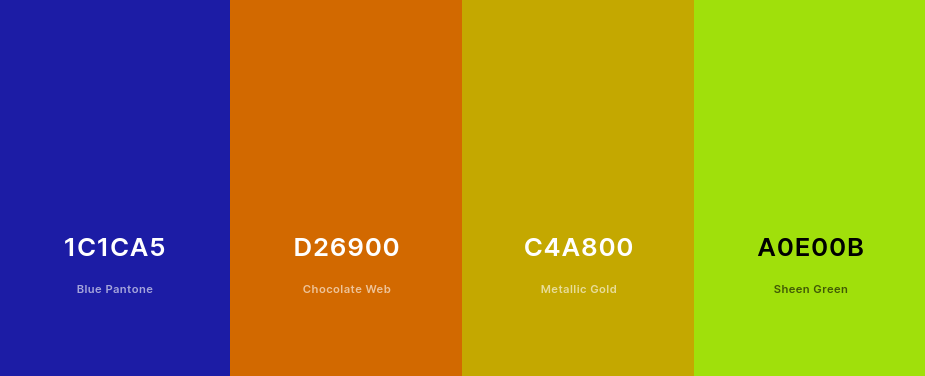
\includegraphics[scale = 0.4]{img/C7/paleta.png}
    \caption{Paleta de colores elegida para la visualización de fractales 2D}
    \label{fig:paleta}
\end{figure}

La paleta de colores \ref{fig:paleta} nos proporciona el gradiente de la imagen \ref{fig:gradiente}, que próximamente podremos ver en nuestros fractales, de manera que los puntos que diverjan antes se acercarán más al azul y los que tarden más se colorearán de un color más parecido al verde.

\begin{figure} [ht]
    \centering
    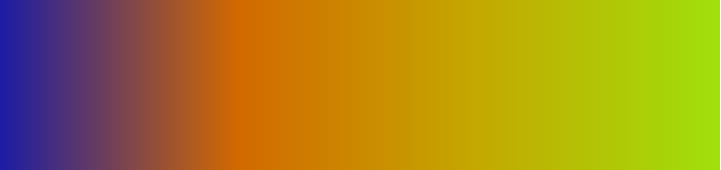
\includegraphics[scale = 0.51]{img/C7/gradiente.png}
    \caption{Gradiente generado por la paleta de colores \ref{fig:paleta}}
    \label{fig:gradiente}
\end{figure}

Con esta decisión tomada, presentamos el código utilizado

\begin{lstlisting}
// Paleta de colores, a partir de un numero 0<=t<=1 y 4 
// colores c1, c2, c3 y c4 devuelve el color 
// correspondiente en el gradiente creado por los cuatro 
// colores.
vec3 palette(float t, vec3 c1, vec3 c2, vec3 c3, vec3 c4) {
  float x = 1.0 / 3.0;
  if (t < x) return mix(c1, c2, t/x);
  else if (t < 2.0 * x) return mix(c2, c3, (t - x)/x);
  else if (t < 3.0 * x) return mix(c3, c4, (t - 2.0*x)/x);
  return c4;
}

// Asignacion de colores, a partir de una variable que define
// si el punto es prisionero o de escape y el numero de 
// iteraciones antes de escapar se calcula y devuelve un color 
// que proximamente se asignara finalmente a gl_FragColor
vec4 computePixelColor(bool escaped, int iterations) {
    return escaped ? vec4(palette(
      float(iterations)/ float(u_maxIterations),
      vec3(0.109,0.109,0.647), // #1C1CA5
      vec3(0.823, 0.411, 0.0), // #D26900
      vec3(0.769, 0.659, 0.0), // #C4A800
      vec3(0.627,0.878,0.043)  // #A0E00B
      ), 
      1.0) : vec4(vec3(0.0,0.0,0.0), 1.0);
}
\end{lstlisting}

Como se puede observar, es una simple interpolación lineal entre los 4 colores que se acaban de presentar, que en GLSL deben codificarse como tripletas RGB donde cada componente está normalizada entre 0 y 1.

\section{Visualizando conjuntos de Julia}
\label{section:grafica-julia}

Tenemos entonces todos los ingredientes para programar la visualización, tan solo falta decidir si el punto que representa el píxel es prisionero o escapa mediante la iteración de $P_{c,m}$. Tras obtener las coordenadas de mundo que se le asignan al píxel mediante el método descrito en la sección \ref{section:pantalla-plano}, debemos iterar la función $P_{c,m}$. Atendiendo al teorema \ref{th:escape}, en caso de que el módulo supere el valor 2 se decide que el punto es de escape. Si esto nunca ocurre y se alcanza el número máximo de iteraciones sin que el módulo sea mayor que 2, entonces se decide que el punto es prisionero (recordemos el pseudocódigo del algoritmo \ref{alg:Julia}). Atendiendo a esta decisión y al número de iteraciones dadas se asigna el color correspondiente como comentamos en la sección \ref{section:colores}. El código GLSL sería el siguiente:

\begin{lstlisting}
// A partir del valor de la semilla z0, la constante c 
// y el exponente m iteramos la funcion P_{c,m}.
void iterateJulia(vec2 z0, vec2 c, int m, 
  out bool escaped, out int iterations) {  
  vec2 z = z0;
  escaped = false;
  for(int i = 0; i < 10000; i++) {
    if(i == u_maxIterations) break;
    iterations = i;
    z = P(z, c, m);
    if (length(z) > 2.0){
      escaped = true;
      break;
    }
  }
}


// A partir del valor de la constante c y el exponente m
// se calcula el punto asociado al pixel, se itera P_{c,m}
// y se devuelve el color en funcion de dicha iteracion.
vec4 Julia(vec2 c, int m) {
  vec2 z0 = get_world_coordinates();
  bool escaped;
  int iterations;
  iterateJulia(z0, c, m, escaped, iterations);
  return computePixelColor(escaped, iterations);
}
\end{lstlisting}

Nótese el uso de los parámetros \verb|out|, que son variables las cuales mantienen el valor que se les haya asignado en la función después del retorno. En este caso, se itera $P_{c,m}$ y se asigna \verb|true| a la variable \verb|escaped| si y solo si la sucesión de iteradas diverge. En caso de que la sucesión diverja, la variable \verb|iterations| almacenaría el número de iteraciones calculadas hasta que el módulo de la iterada supere a $2$. 

Por último, desde la función \verb|main|, llamamos a esta función recién presentada, le asignamos el color que devuelve a \verb|gl_FragColor| y obtenemos los resultados que se presentan en las imágenes \ref{fig:julia-webgl}.  

\begin{lstlisting}
gl_FragColor = Julia(u_juliaSetConstant, u_order);
\end{lstlisting}

\begin{figure}[ht]
    \centering
    \begin{tabular}{ccc}
      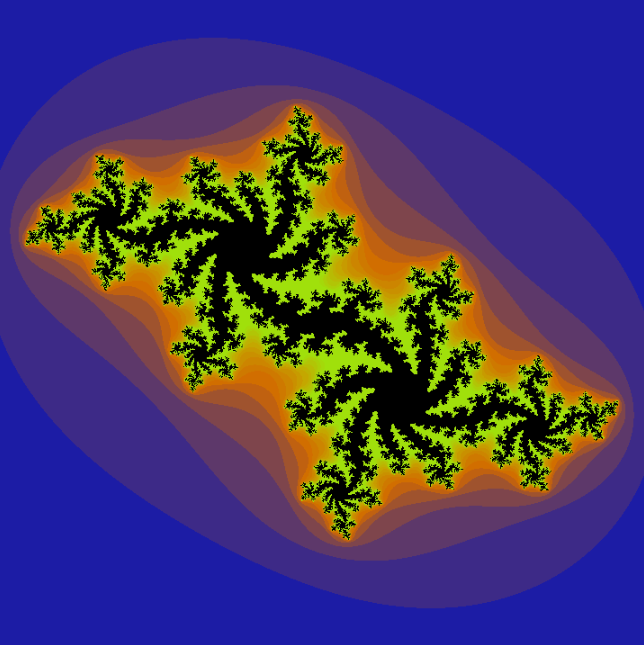
\includegraphics[scale=0.2]{img/C7/julia-1.png} &   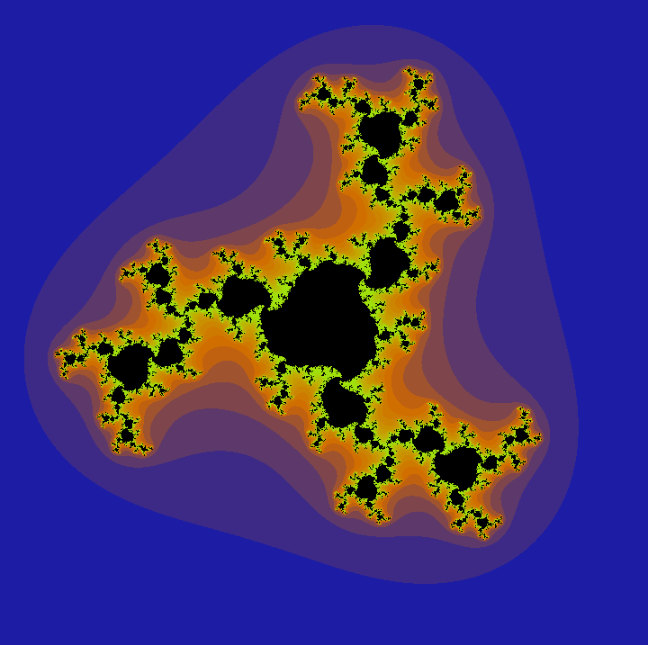
\includegraphics[scale=0.2]{img/C7/julia-2.png} &   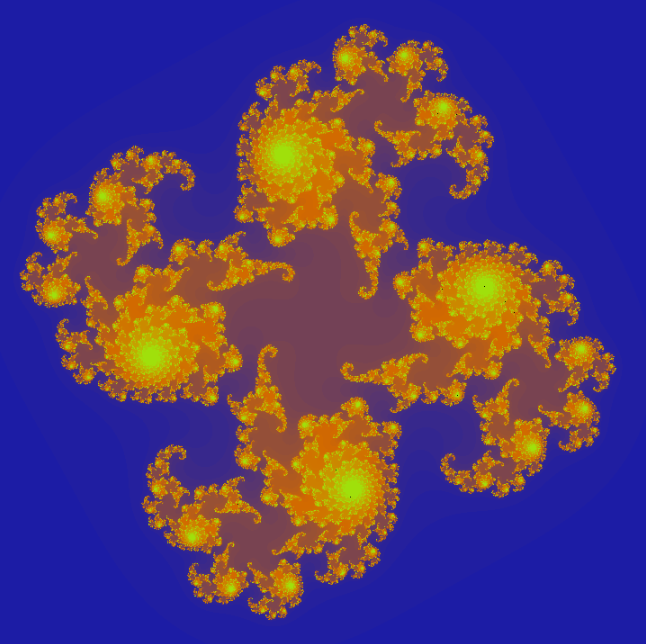
\includegraphics[scale=0.2]{img/C7/julia-3.png} \\
    (a) $z^2-0.38+0.62i$ & (b) $z^3+0.62+0.5i$ & (c) $z^4-0.24+0.5i$ \\[6pt]
    \end{tabular}
    \caption{Generación de algunos conjuntos de Julia con WebGL}
    \label{fig:julia-webgl}
\end{figure}

\section{Visualizando conjuntos de Mandelbrot}

Ya hemos visto la metodología a utilizar si queremos visualizar conjuntos de Julia y, como es de esperar, la metodología para graficar conjuntos de Mandelbrot $\mathcal{M}_m$ no es muy distinta. Recordamos que, tal y como afirmamos en las secciones \ref{section:Mandelbrot} y \ref{subsection:julia-mandelbrot-generalizados} el conjunto de Mandelbrot $\mathcal{M}_m$ se componía de aquellos elementos $c\in\C$ tales que el conjunto de Julia $\mathcal{J}_c$ es conexo, o equivalentemente, de aquellos cuya sucesión $\{P_{c,m}^n(0)\}$ no diverge.

La idea consiste por tanto en obtener las coordenadas de mundo del píxel, iterar la función $P_{c,m}$ tomando $z_0=0$ como semilla y observar qué sucede, recordemos el algoritmo \ref{alg:Mandelbrot}. Por la proposición \ref{prop:mandelbrot-escape} afirmamos que en el momento que una iterada supere en módulo a 2, entonces la sucesión de iteradas es divergente. Por tanto, almacenamos en una variable el número de iteradas que se han calculado antes de que el módulo de la sucesión supere a 2 en caso de que lo haga. Si esto no ocurre, se etiqueta al punto como prisionero y por tanto el punto pertenece a $\mathcal{M}_m$. De nuevo, la forma de asignar un color al píxel depende de si la sucesión diverge o no y del número de iteraciones hasta decidir que diverge en dicho caso. El código GLSL por tanto es el siguiente:

\begin{lstlisting}
// A partir de la constante c, el exponente m y 
// tomando como semilla z=0 se itera P_{c,m} 
void iterateMandelbrot(vec2 c, int m, 
  out bool escaped, out int iterations) {
    
  vec2 z = vec2(0.0);
  escaped = false;
  for (int i = 0; i < 10000; i++) {
    if (i == u_maxIterations) break;
    iterations = i;
    z = P(z, c, m);
    if (length(z) > 2.0) {
      escaped = true;
      break;
    }
  }
}

// A partir del exponente m se calcula el punto asociado al
// pixel, se itera y se devuelve el color asociado.
vec4 Mandelbrot(int m) {
  vec2 c = get_world_coordinates();
  bool escaped;
  int iterations;
  iterateMandelbrot(c, m, escaped, iterations);
  return computePixelColor(escaped, iterations);
}
\end{lstlisting}

Vemos la analogía entre las funciones \verb|iterateJulia| y \verb|Julia| con las funciones \verb|iterateMandelbrot| y \verb|Mandelbrot|, estando las primeras presentadas en la sección \ref{section:grafica-julia}. La diferencia fundamental se encuentra en que mientras en los conjuntos de Julia fijamos un $c\in\C$ y usamos el complejo asociado al píxel como semilla en el caso del conjunto de Mandelbrot usamos siempre $z_0=0$ como semilla y tomamos como $c$ el complejo que representa el píxel.

Por tanto, ya solo falta llamar a esta función desde \verb|main|, asignarle el valor que devuelve a \verb|gl_FragColor| y podremos ver el conjunto de Mandelbrot en detalle. Presentamos algunas imágenes de detalles del mismo, a la vez que animamos a revisitar las imágenes \ref{fig:mandelbrot-intro}, las cuales también se han obtenido mediante WebGL.

\begin{lstlisting}
gl_FragColor = Mandelbrot(u_order);
\end{lstlisting}

\begin{figure}[ht]
    \centering
    \begin{tabular}{ccc}
      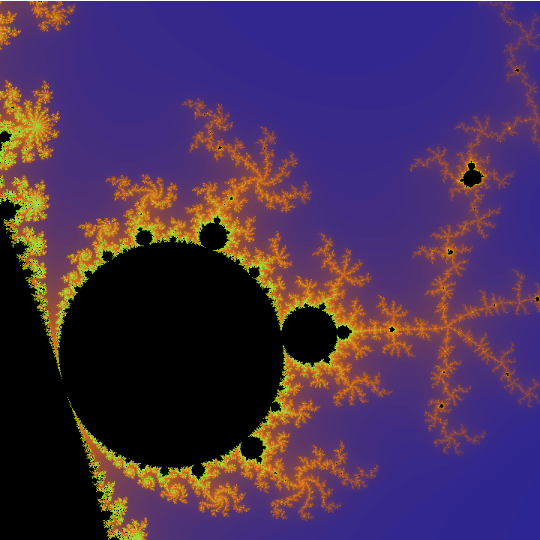
\includegraphics[scale=0.23]{img/C7/mandelbrot-1.png} &   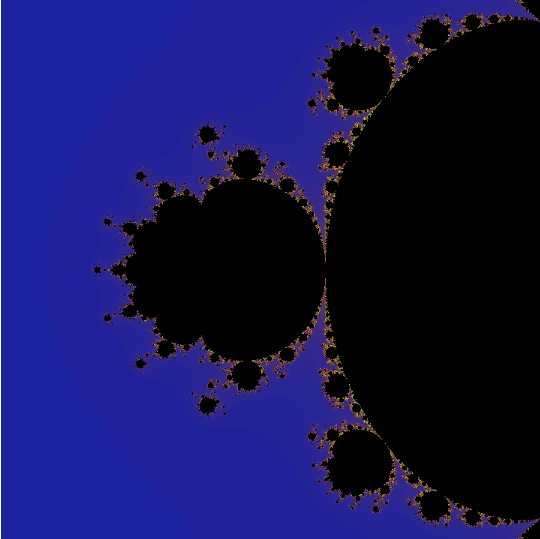
\includegraphics[scale=0.23]{img/C7/mandelbrot-2.png} &   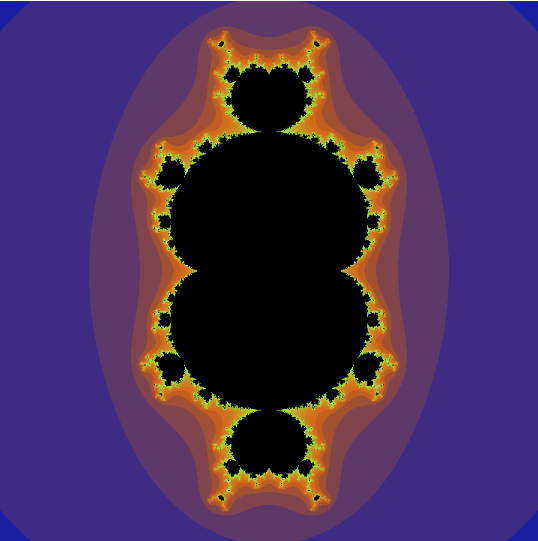
\includegraphics[scale=0.23]{img/C7/mandelbrot-3.png} \\
    (a) Detalle de $\mathcal{M}_2$ & (b) Detalle de $\mathcal{M}_8$ & (c) $\mathcal{M}_3$ \\[6pt]
    \end{tabular}
    \caption{Representación de algunos conjuntos de Mandelbrot con WebGL}
    \label{fig:mandelbrot-webgl}
\end{figure}

\newpage

\section{Alternando conjuntos de Julia y Mandelbrot}
\label{section:alternando}

Finalmente, queremos dotar a nuestra web de la posibilidad de alternar qué fractal visualizar (Julia o Mandelbrot) y poder ajustar los parámetros a nuestro gusto. Para ello introducimos en el fragment Shader una variable \verb|uniform| entera que, en caso de valer 0 se visualizaría el conjunto de Mandelbrot y en caso de valer 1 se visualizaría el conjunto de Julia.

\begin{lstlisting}
// Graficar conjunto de Julia o de Mandelbrot
uniform int u_fractal;

// ... 

void main() {
  vec4 color;
  if(u_fractal == 0){
    color = Mandelbrot(u_order);
  }
  else{
    color = Julia(u_juliaSetConstant, u_order);
  }
  gl_FragColor = color;
}
\end{lstlisting}

\section{Supersampling Antialiasing}
\label{section:SSAA-2D}

Para terminar este capítulo, introduciremos una técnica que aportará realismo y calidad a nuestras imágenes. El aliasing es un efecto que ocurre en muchas aplicaciones gráficas debido a la discretización que se realiza de una imagen real en un subconjunto finito de píxeles. Por ejemplo, a no ser que una línea recta sea totalmente vertical u horizontal, se presentará con sobresaltos impropios de una línea recta (véase imagen \ref{fig:no-antialiasing-3D}).Por su parte, el \textit{antialiasing} es un conjunto de técnicas que nos permite evitar este efecto mediante el suavizado de bordes. Por ejemplo, fíjese en la imagen \ref{fig:no-antialiasing-2D}, de $\mathcal{J}_{-0.53 + 0.53i}$. En ella se pueden observar irregularidades, como por ejemplo pequeños puntos negros o píxeles consecutivos de colores muy distintos.

\begin{figure} [ht]
  \centering
  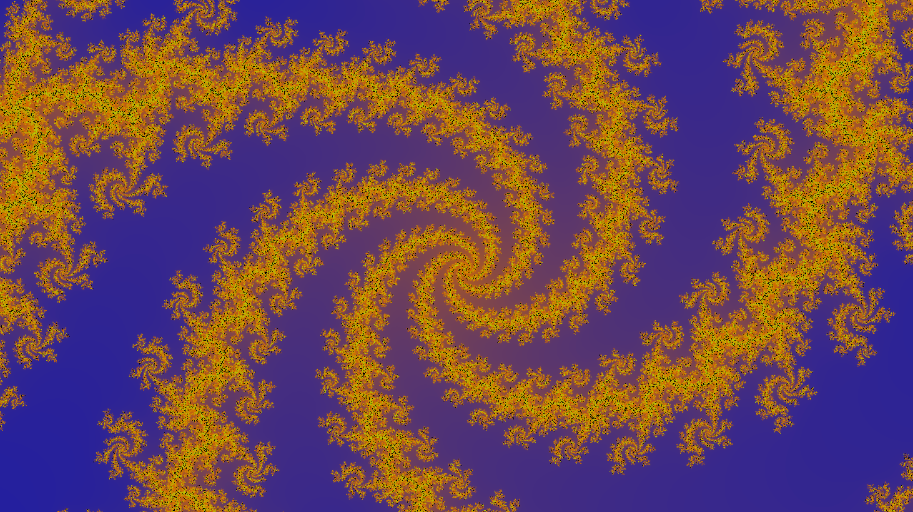
\includegraphics[width=130mm]{img/C7/no-antialiasing.png}
  \caption{Detalle de $\mathcal{J}_{-0.53 + 0.53i}$ antes de aplicar antialiasing}
  \label{fig:no-antialiasing-2D}
\end{figure}

Una forma simple de corregir estos efectos se consigue teniendo en cuenta que se está identificando cada píxel con un único punto del plano, cuando realmente en cada píxel hay infinitos puntos. Podría incluso ocurrir que el conjunto de Julia atravesara el píxel de forma que la mayor parte de sus puntos sean de escape pero el que evalúa el algoritmo es prisionero, coloreando el píxel de color negro cuando realmente no todos los puntos que lo componen son prisioneros. Una solución sencilla a este impedimento es aplicar la técnica popularmente conocida como \textit{Supersampling Antialiasing} (SSAA). El SSAA consiste en calcular más de un punto por píxel, de forma que se cubra una región más representativa del mismo y se promedie el color que devuelve el algoritmo en cada uno de los puntos.

Fijémonos en la figura \ref{fig:pantalla-antialiasing} (a), en la cual representamos una pantalla de $5\times 3$ píxeles y cada punto señalado sería un punto del plano complejo que iteraríamos y calcularíamos el color asociado según las técnicas implementadas hasta el momento. Para calcular más de un punto, fijamos un número natural $n\in\N$ y programaremos la forma de calcular $n^2$ puntos en cada píxel, tal y como vemos en la imagen \ref{fig:pantalla-antialiasing} (b) con $n=2$.

\begin{figure}[ht]
    \centering
    \begin{tabular}{cc}
        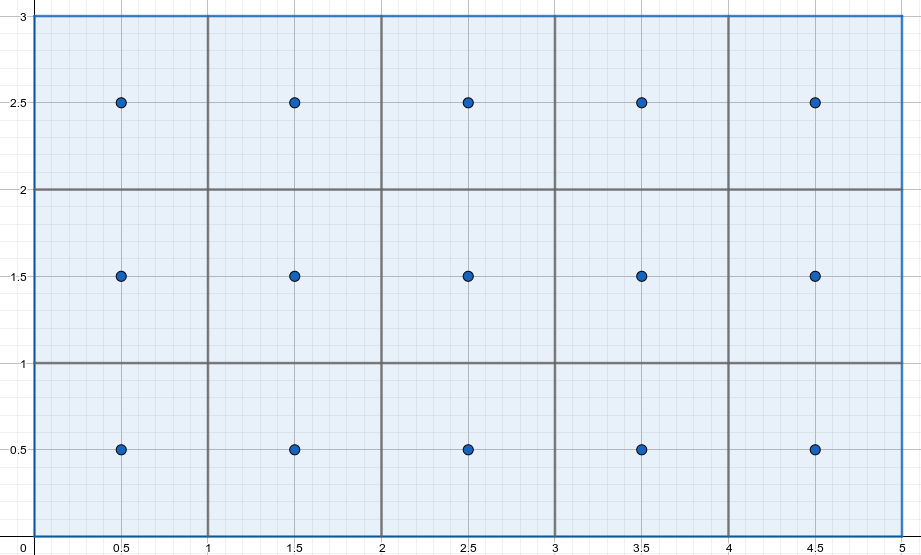
\includegraphics[scale=0.20]{img/C7/pixeles-sin-antialiasing.png} &
      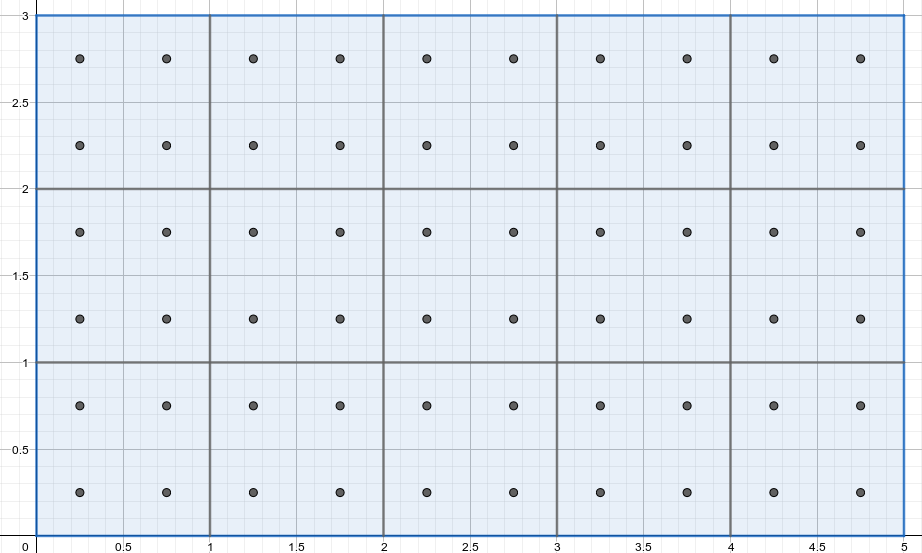
\includegraphics[scale=0.20]{img/C7/pixeles-con-antialiasing.png} \\    
    (a) Sin antialiasing & (b) Con antialiasing  \\
    \end{tabular}
    \caption{Representación de los rayos que se lanzan a una pantalla}
    \label{fig:pantalla-antialiasing}
\end{figure}

Por tanto, ahora, en lugar de calcular las ``coordenadas de mundo de cada píxel'', a las cuales nos referíamos como las coordenadas de mundo del punto situado en el centro del píxel, ahora debemos calcular, por cada píxel, $n^2$ coordenadas. 

Recordamos, del código de la función \verb|get_world_coordinates| presentado en la sección \ref{section:pantalla-plano}, 

que utilizamos las variables \verb|u,v| como las coordenadas de dispositivo normalizadas en $[0,1]$, es decir:

\begin{lstlisting}
// ... 
vec2 uv = (gl_FragCoord.xy + vec2(0.5)) / 
          vec2(float(nx), float(ny));
float u = uv.x;
float v = uv.y;
\end{lstlisting}

Si ahora en lugar de utilizar un punto por píxel situado en centro del mismo deseamos tener $n^2$ puntos uniformemente distribuidos por la superficie del píxel, tenemos que dividir su ancho en $n$ intervalos, análogamente el alto. Por tanto, dividimos cada píxel en una cuadrícula $n\times n$ donde cada fragmento mide $h_w:=\frac{1}{n_x\cdot n}$ en anchura y de $h_h:=\frac{1}{n_y\cdot n}$ en altura. Tras esto, deberíamos sumar $\frac{1}{2}h_w$ en ancho y $\frac{1}{2}h_h$ en alto, para así tener dicha cuadrícula centrada en el píxel, véase la imagen \ref{fig:SSAA}.

\begin{figure} [ht]
  \centering
  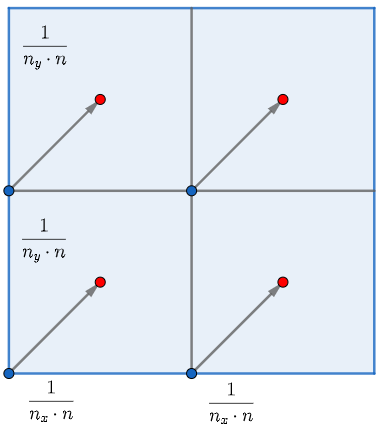
\includegraphics[scale = 0.45]{img/C7/SSAA.png}
  \caption{Construcción de los puntos por píxel en SSAA}
  \label{fig:SSAA}
\end{figure}

Seguidamente, calculamos los $n^2$ colores, uno por cada punto que utilicemos. Por cada punto, iteramos la función $P_{c,m}$ igual que en las secciones anteriores y que en los algoritmos \ref{alg:Julia} y \ref{alg:Mandelbrot} y calculamos el color que le corresponde, de forma que sumamos los $n^2$ colores que se calculan.  Finalmente, dividimos esta suma entre $n^2$, obteniendo así el color promedio del píxel, siendo este el valor que se asignaría finalmente a \verb|gl_FragColor|.

La forma de hacer este cálculo es iterando un índice $i=0,\dots,n^2$. Para a partir del índice $i$ obtener la coordenada correspondiente podemos dividir el conjunto $\sigma_{n^2}=\{0,1,\dots,n^2-1\}$ en $n$ conjuntos de $n$ elementos cada uno, de forma que
$$
\sigma_{n^2} = \bigcup_{k=0}^{n-1} \{nk, nk+1, \dots, nk+n-1\}.
$$

Cada subconjunto de $\sigma_{n^2}$ representa una fila de puntos del píxel. Por tanto, aplicando la división entera, $i/n$ será la fila e $i\%n$ la columna. Por lo que habría que sumar $(i/n)h_w + \frac{1}{2}h_w$ a la coordenada anchura inicial e $(i\%n)h_h+ \frac{1}{2}h_h$ a la altura para obtener la coordenada del punto $i$-ésimo.

Para ello, modificamos la función \verb|get_world_coordinates| para que acepte el índice $i$ (\verb|int i|) y el valor $n$ (\verb|int nSamples|) como parámetros y calcule las coordenadas de mundo del punto $i$-ésimo del píxel.

\begin{lstlisting}
vec2 get_world_coordinates(int i, int nSamples) {

  int nx = 1280, ny = 720; // Canvas size (pixels)
  float r = 16.0/9.0;      // Ratio width/height = 16/9
  float h = 4.0, w = r * h;  // Image size (units) 

  // Incrementos
  float hw = 1.0 / (float(nx * nSamples)),
        hh = 1.0 / (float(ny * nSamples));

  int x =  i/nSamples;
  int y =  i - nSamples*x;

  // Coordenadas de dispositivo normalizadas en [0,1]x[0,1]
  vec2 uv = (gl_FragCoord.xy) / 
            vec2(float(nx), float(ny));
  float u = uv.x + float(x) * hw + 0.5 * hw,
        v = uv.y + float(y) * hh + 0.5 * hh;
  
  return u_zoomCenter + vec2(u*w - w/2.0, v*h - h/2.0) * u_zoomSize;
}
\end{lstlisting}

Finalmente, en las funciones \verb|Julia| y \verb|Mandelbrot|, en lugar de hacer una única llamada a la función \texttt{get\_world\_coordinates()}, hacemos $n^2$ llamadas a \texttt{get\_world\_coordinates(i, nSamples)}, fijando previamente el valor de $n$ (\verb|nSamples|). Sumamos los $n^2$ colores que se calculan en cada muestra y finalmente se devuelve el promedio. Mostramos el código de la función \verb|Julia|, ya que el de \verb|Mandelbrot| es totalmente análogo.

\begin{lstlisting}
vec4 Julia(vec2 c, int n) {
  vec4 sum_colors = vec4(0.0, 0.0, 0.0, 1.0);
  int nSamples = 3; // Se calcularian 3^2 = 9 colores
  for(int i = 0; i < 1000; i++) {
    if(i == nSamples*nSamples) break;
    vec2 z0 = get_world_coordinates(i, nSamples);
    bool escaped;
    int iterations;
    iterateJulia(z0, c, n, escaped, iterations);
    sum_colors += computePixelColor(escaped, iterations);
  } 
  return sum_colors/float(nSamples*nSamples);
}
\end{lstlisting}

El resultado tras aplicar esta modificación en $\mathcal{J}_{-0.53 + 0.53i}$, que es el conjunto que aparece en la imagen \ref{fig:no-antialiasing-2D}, es la imagen \ref{fig:antialiasing-2D}. Fijémonos como la sensación de irregularidad desaparece, dando apariencia más suavizada, mejorando notablemente la calidad de la imagen.

\begin{figure} [ht]
  \centering
  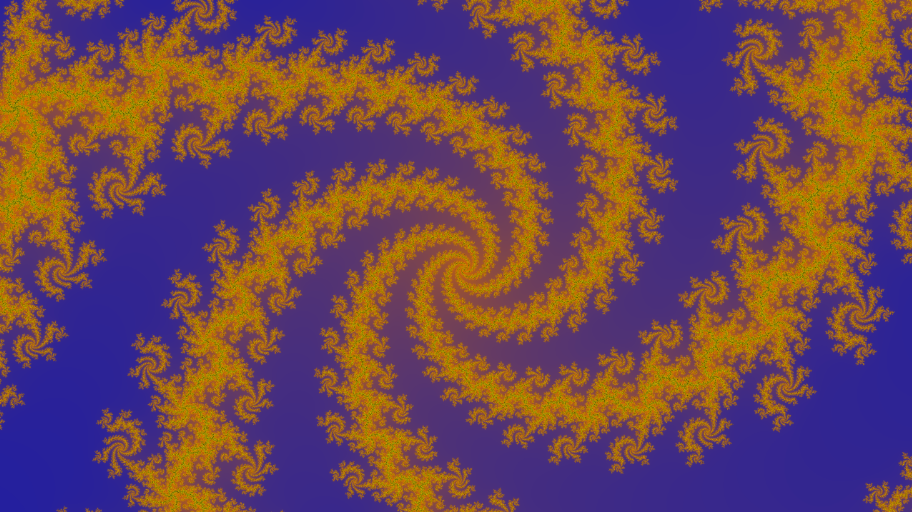
\includegraphics[width=130mm]{img/C7/antialiasing.png}
  \caption{Detalle de $\mathcal{J}_{-0.53 + 0.53i}$ tras aplicar SSAA}
  \label{fig:antialiasing-2D}
\end{figure}

El principal y mayor inconveniente que presenta esta técnica es que, como se puede imaginar, es $n^2$ veces más costosa que utilizar un único punto por píxel, por lo que se ralentiza mucho la ejecución. Sin embargo, si se desea una imagen concreta con parámetros muy claros y no tanto la interacción es una buena herramienta, pues proporciona un nivel de detalle mucho mayor.

Precisamente por este costo, se incluye en el software la posibilidad de decidir si se desea o no aplicar SSAA, y en caso afirmativo, cuántos rayos por píxel se desean trazar. Esto se consigue mediante dos variables \verb|uniform|. Una de ellas es booleana, su nombre es \verb|u_antialiasing|, que en caso de valer \verb|true| se aplicaría antialiasing y en caso contrario se utilizaría un único punto por píxel. Para ello utilizamos la otra variable \verb|uniform|, que es entera y su nombre es \verb|u_nSamples|, que es la análoga a la $n$ que hemos utilizado en las explicaciones. En caso de que \verb|u_antialiasing| tenga el valor \verb|false|, \verb|u_nSamples| tendrá el valor $1$, en caso contrario tendrá el valor que decida el usuario.  

\begin{lstlisting}
uniform bool u_antialiasing;
uniform int u_nSamples;
// ...
vec4 Julia(vec2 c, int n) {
  vec4 sum_colors = vec4(0.0, 0.0, 0.0, 1.0);
  // int nSamples = 3;
  int nSamples = u_antialiasing ? u_nSamples : 1;
  // ... 
}
\end{lstlisting}
